\question{Газовый разряд. Виды и характеристики газового разряда. Рождение и
  исчезновение носителей зарядов}

В обыкновенных условиях, то есть при отсутствии внешнего воздействия, газ
является диэлектриком. Ток будет течь только при наличии внешнего ионизатора,
например, космического излучения. Если ионизатор убрать, то ток исчезнет. Такой
разряд называется \emph{несамостоятельным} (рис.~\pic{32VAC}-I).
\begin{figure}[h!]
  \center
  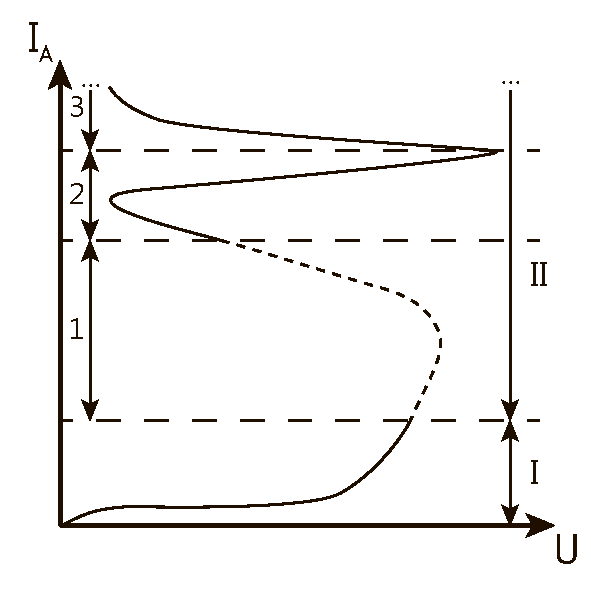
\includegraphics[width=.3\textwidth]{32_VAC} \hspace{1em}
  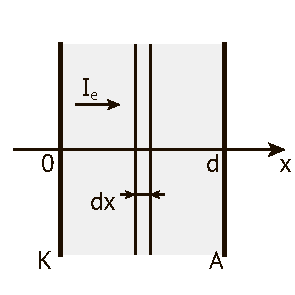
\includegraphics[width=.3\textwidth]{32_Townsend} \hspace{1em}
  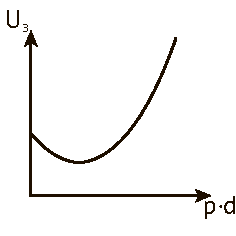
\includegraphics[width=.3\textwidth]{32_U_light} \\
  \parbox{.3\textwidth}{\caption{ВАХ газового разряда} \label{pic32VAC}}
    \hspace{1em}
  \parbox{.3\textwidth}{\caption{К описанию эффекта Таунсенда}
    \label{pic32Townsend}} \hspace{1em}
  \parbox{.3\textwidth}{\caption{Зависимость \( U_\text{з}(p \cdot d\))}
    \label{pic32U}} \\
  \parbox{.37\textwidth}{\footnotesize I~-- несамостоятельный разряд,
    II~-- самостоятельный разряд; 1~-- переходная область, 2~-- тлеющий
    разряд, 3~-- дуговой разряд}
  \parbox{.62\textwidth}{\ }
\end{figure}

При повышении разности потенциалов между анодом и катодом энергия электронов
будет увеличиваться, и при достижении некоторого напряжения этой энергии будет
достаточно, чтобы при столкновении электронов с нейтральными атомами произвести
ионизацию. Ток увеличивается, это явление называется газовым усилением. Однако
если убрать внешний ионизатор, ток упадет до нуля, следовательно, такой разряд
также является несамостоятельным.

При дальнейшем повышении напряжения, положительные ионы, попадая на катод,
начинают вызывать вторичную эмиссию. При этом, даже если убрать внешний
ионизатор, ток не прекратится. Такой разряд называется \emph{самостоятельным}
(рис.~\pic{32VAC}-II). Область~2 на ВАХ называется \emph{тлеющим разрядом}.

При дальнейшем увеличении напряжения ионы будут разогревать катод, проявится
явление термоэлектронной эмиссии (область~3). Такой разряд называется
\emph{дуговым}.

\subquestion{Эффект Таунсенда}

Эффектом Таунсенда называется переход разряда из несамостоятельного в
самостоятельный. Пусть \( \alpha \)~-- коэффициент объемной ионизации, равный
количеству электронно-ионных пар, образуемых одним электроном на единице пути.

Коэффициент \( \alpha \) зависит от давления \( p \) и напряженности
электрического поля \( E \).

Выделим в газовом промежутке слой толщиной \( dx \) (рис.~\pic{32Townsend}).
Один электрон, пролетая этот слой, создаст \( \alpha\,dx \) электронно-ионных
пар. Если плоскость \( x = \const \) пересекает ток электронов \( I_e \), то в
слое \( dx \) он возрастет на величину
\begin{equation}
  dI_e = \alpha I_e\,dx.
  \label{eq32dIe}
\end{equation}

Если положить, что \( U = \const \), то \( \alpha = \const(x) \). Проинтегрируем
\eqref{eq32dIe}:
\begin{equation}
  I_e = I_e(0)e^{\alpha x},
  \label{eq32Ie}
\end{equation}
где \( I_e(0) \)~-- прикатодный ток (ток, создаваемый внешним ионизатором).

Чтобы разряд не прекращался, необходимо поддерживание тока \( I_e(0) \) самим
разрядом, то есть возникал бы поток положительно заряженных ионов, движущихся к
катоду.

Данный ток легко определить из закона сохранения заряда:
\[
  I_i(0) = I_e(d) - I_e(0); \qquad I_i(0) = I_e(0) \Big[ e^{\alpha d} - 1 \Big].
\]

Пусть каждый пришедший на катод ион выбивает в среднем \( \gamma(p, E) \)
вторичных электронов. Следовательно, из катода начнет эмитироваться ток
вторичных электронов \( I_2 \):
\[
  I_2 = \gamma I_i(0) = \gamma I_e(0) \Big[ e^{\alpha d} - 1 \Big].
\]

Таким образом, полный ток, эмитируемый с катода:
\[
  I_e(0) = I_1 + I_2,
\]
где \( I_1 \)~-- ток, вызываемый внешним ионизатором.

\[
  I_e(0) = I_1 + \gamma I_e(0) \Big[ e^{\alpha d} - 1 \Big]; \quad
    I_e(0) = \frac{I_1}{1 - \gamma(e^{\alpha d} - 1)}; \quad
    I_e(d) = \frac{I_1 e^{\alpha d}}{1 - \gamma(e^{\alpha d} - 1)}.
\]

Если убрать внешний ионизатор, то \( I_1 \to 0 \) и \( I_e(d) \to 0 \). Но
можно подобрать \( \gamma \) и \( \alpha \) таким образом, чтобы
\(
  \gamma \Big[ e^{\alpha d} - 1 \Big] \to 1
\).

Величину \( \mu = \gamma \Big[ e^{\alpha d} - 1 \Big] \) называют коэффициентом
воспроизводства. \( \mu = 1 \) является критерием Таунсенда~-- критерием
перехода из несамостоятельного в самостоятельный.

Так как давление \( p \) во многих случаях остается постоянным, то
\( \gamma = \gamma(U) \), \( \alpha = \alpha(U) \). Потенциал, при котором
происходит переход разряда из несамостоятельного в самостоятельный, называется
потенциалом зажигания \( U_\text{з} = U_\text{з}(p \cdot d) \) (рис.~\pic{32U}).

\subquestion{Характеристики газового разряда}

\hspace{1.5em}\textbf{Средняя длина свободного пробега}

Средняя длина свободного пробега \( \lambda \)~-- это среднее расстояние,
которое проходит электрон между соударениями с нейтральными атомами.

Функцию распределения длин свободных пробегов можно получить в предположении
равновероятности всех направлений и при условии равенства по абсолютной величине
скоростей всех частиц. Пусть \( P(x) \)~-- вероятность того, что длина
свободного пробега превышает \( x \). Тогда вероятность того, что столкновение
произойдет в слое от \( x \) до \( x + dx \) пропорциональна толщине слоя:
\( \alpha\,dx \). Соответственно, вероятность того, что столкновение не
произойдет, равна \( 1 - \alpha\,dx \). Вероятность того, что столкновение
не произойдет при прохождении частицы пути длиной \( x + dx \), равна
произведению \( 1 - \alpha\,dx \) и \( P(x) \):
\[
  P(x)(1 - \alpha\,dx) = P(x + dx) \approx P(x) + \pder{P}{x}\,dx,
    \text{ или } \pder{P}{x} = -\alpha P(x).
\]

Интегрируем, учитывая тот факт, что\( \lambda > 0 \) и, следовательно,
\( P(0) = 1 \). Получаем
\[
  P(x) = e^{-\alpha x}.
\]

Тогда вероятность того, что \( \lambda \) находится в интервале
\( [x, x + dx] \), равна
\[
  P(x) - P(x + dx) = -\pder{P}{x} = f(x)\,dx = \alpha e^{-\alpha x}\,dx,
\]
где \( f(x) \) является функцией распределения длин свободного пробега. Средняя же
длина находится из известного соотношения:
\begin{equation}
  \average{\lambda} = \int\lni xf(x)\,dx = \alpha\int\lni xe^{-\alpha x}\,dx =
    \frac{1}{\alpha}.
  \label{eq32averagel}
\end{equation}

\textbf{Эффективное поперечное сечение столкновения}

Вероятность того, что электрон столкнется с атомами, можно описать и при помощи
понятия эффективного поперечного сечения столкновения \( \sigma \). Под ним 
понимается величина, определяемое как число столкновений \( d\nu \),
происходящих в единичном объеме \( dV \) в единичном интервале времени \( dt \):
\[
  \sigma = \frac{d\nu}{v_{12} n_e n\,dV\,dt},
\]
где \( n_e \)~-- концентрация электронов, \( n \)~-- концентрация атомов,
\( v_{12} = \abs{\vec{v}_2 - \vec{v}_1} \)~-- разность скоростей пучков
налетающих частиц.

Рассмотрим однородный по скорости пучок электронов, проходящих через газ.
Вероятность столкновения для каждого электрона в слое толщиной \( dx \)
пропорциональна \( n\sigma\,dx \). Будем считать, что электроны, испытавшие
столкновения, покидают пучок. Тогда относительное изменение силы тока пучка
\begin{equation}
  \frac{dI}{I} = n\sigma\,dx, \text{ интегрируя получим }
    I = I_0 e^{n\sigma x},
  \label{eq32I(x)}
\end{equation}
где \( I_0 \)~-- начальный ток пучка, \( I \)~-- ток пучка после прохождения им
расстояния \( x \). Сравнивая \eqref{eq32Ie} и \eqref{eq32I(x)}, видно, что
\( \alpha = n\sigma \), а средняя длина свободного пробега (из
\eqref{eq32averagel}): \( \average{\lambda} = 1 / (n\sigma) \).

\textbf{Транспортные сечение и длина}

При соударениях электронов с нейтральными атомами электроны могут
потерять свою энергию и изменить свой импульс. Рассмотрим соударение электрона
массой \( m \) с неподвижным атомом массой \( M \) (рис.~\pic{32transport}):
\[
  \left\{
    \begin{array}{l}
      p_a^2 = p^2 + {p'}^2 - 2pp'\cos\theta \\
      \dfrac{p^2}{2m_e} = \dfrac{{p'}^2}{2m_e} + \dfrac{p_a^2}{2M}.
    \end{array}
  \right.
\]

Так как \( m_e \ll M \), то
\[
  \abs{\vec{p}} \approx \abs{{\vec{p}}\,'}, \quad
    p^2 - {p'}^2 \approx 2p \left( p - p' \right), \quad
    pp' \approx p^2 \quad \text{ и } \quad
    p^2 + {p'}^2 \approx 2p^2.
\]

Тогда, подставляя \( p_a^2 \) из первого уравнения во второе, получим
\[
  2p\frac{M}{m_e} \Big( p - p' \Big) = 2p^2 - 2p^2\cos\theta; \quad
    \frac{p - p'}{p} = \frac{m_e}{M} \Big( 1 - \cos\theta \Big); \quad
    \frac{\D p}{p} = -\frac{m_e}{M} 1 - \cos\theta.
\]

\begin{figure}[h!]
  \center
  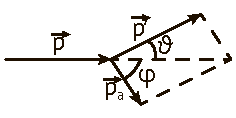
\includegraphics[width=.3\textwidth]{32_transport} \\
  \caption{К выводу транспортного сечения}
  \label{pic32transport}
\end{figure}

Для характеристики влияния столкновений на движение частиц вводят интегральное
сечение, характеризующее изменение импульса и энергии при упругих столкновениях:
\[
  \sigma_d = \iint \Big( 1 - \cos\theta \Big) I(\theta, \phi) \sin\theta\,
    d\theta\,d\phi,
\]
где \( I(\theta, \phi) \)~-- изначальное распределение тока по углам,
\( \sigma_d \)~-- сечение передачи импульса (транспортное сечение).

По аналогии с \eqref{eq32averagel} вводят среднюю длину передачи импульса
(транспортную длину):
\[
  \lambda_d = \frac{1}{n\sigma_d}.
\]

\subquestion{Процессы потери электронов}

\hspace{1.5em}\textbf{Диффузия}

Закон Фика гласит: \( \vec{M} = -D\,\gradient\rho \), где \( M \)~-- масса
вещества, диффундирующего в единицу времени через единичную площадку,
\( \rho \)~-- плотность вещества.

Домножим на \( e \) и разделим на \( m_e \):
\begin{equation}
  \vec{j} = D^* \gradient n,
  \label{eq32diff}
\end{equation}
где \( n \)~-- объемная плотность заряда, \( j \)~-- плотность тока.

С другой стороны, есть уравнение непрерывности:
\begin{equation}
  \der{n}{t} - \divergence\vec{j} - Q = 0,
  \label{eq32nobreak}
\end{equation}
где \( Q = nq_i \)~-- скорость образования или потери электронов в рассматриваемом
объеме, \( q_i \)~-- скорость образования или потери электронов в рассматриваемом
объеме, отнесенная к одному электрону.

Подставим \eqref{eq32diff} в \eqref{eq32nobreak}
\[
  \pder{n}{t} = D^*\D n + nq_i; \qquad
    \frac{1}{n}\pder{n}{t} - q_i = \frac{D^*}{n}\D n.
\]

Поскольку в левой части стоит производная по времени, а с правой~-- по
координатам, то, чтобы решение существовало при любых координатах и времени,
каждая из частей должна быть равна некоторой константе. Обозначим ее
\( -\gamma \). Получаем систему уравнений:
\[
  \left\{
    \begin{array}{l}
      \displaystyle\pder{n}{t} = (q_i - \gamma)n; \\[.6em]
      \D n + \dfrac{\gamma}{D}n = 0.
    \end{array}
  \right.
\]

Проинтегрируем первое уравнение системы, получим
\(
  n(t) = n_0 e^{(q_i - \gamma)t}
\).

Для того, чтобы проинтегрировать второе уравнение, сделаем ряд допущений:
\begin{itemize}
  \item допустим, что рассматриваемая область является параллелепипедом
    размерами \( a\times b\times c \);
  \item допустим, что на границах \( n = 0 \).
\end{itemize}

Тогда
\[
  n(x, y, z) = n_1\sin\frac{\pi x}{a} \sin\frac{\pi y}{b} \sin\frac{\pi z}{c};
    \quad \frac{\gamma}{D^*} = \frac{\pi^2}{a^2} + \frac{\pi^2}{b^2} +
    \frac{\pi^2}{c^2}.
\]

Если рассматриваемая система является плоским диодом, то \( b\to\infty \) и
\( c\to\infty \), и тогда
\[
  \gamma = \frac{\pi^2}{a^2}D^*; \quad
    \frac{\gamma}{D^*} = \frac{1}{\Lambda^2}; \quad
    n(t) = n_0 e^{\left( q_i - \frac{\pi^2}{a^2}D^* \right)t} =
    n(t) = n_0 e^{\left( q_i - \frac{D^*}{\Lambda^2} \right)t},
\]
где \( \Lambda \)~-- характерная диффузионная длина.

\textbf{Прилипание электронов к нейтральным атомам}

Из-за того, что масса атомов газа много больше массы электрона, то система
обладает малой подвижностью. Поэтому, хоть атом с <<прилипшим>> к нему
электроном и имеет отрицательный заряд, он будет двигаться к аноду с очень малой
скоростью. Из-за этого этот процесс эквивалентен потере электронов.

Введем коэффициент \( \alpha_\text{п} \)~-- число прилипаний на единицу длины.
Тогда
\[
  dn = -\alpha_\text{п}n\,dx; \qquad n = n(0)e^{-\alpha_\text{п}x}.
\]

\textbf{Рекомбинация}

Рекомбинация~-- процесс потери электронов при их столкновении с положительными
ионами.

Когда происходит рекомбинация, плотность положительных ионов и электронов
изменяется, а скорость этого изменения пропорциональна количеству частиц каждого
рода, так что
\[
  \der{n_+}{t} = \der{n_e}{t} = -\alpha_r n_+ n_e,
\]
где \( \alpha_r \)~-- коэффициент рекомбинации. Обычно \( n_+ = n_e = n \),
тогда
\[
  \der{n}{t} = -\alpha_r n^2; \qquad
    \frac{1}{n} = \alpha_r t + \frac{1}{n_0},
\]
где \( n_0 \)~-- начальная плотность частиц.

Отсюда
\(
  \alpha_r = \dfrac{1}{t} \left( \dfrac{1}{n} - \dfrac{1}{n_0} \right)
\).
